\section{Introduction}
% 
Nowadays, to decrease wildfire caused economical loss and ensure human life safety, the concepts of wildfire management are being more and more accepted \cite{tymstra2020wildfire}. Unmanned aerial vehicles (UAV) is thought one of the most efficient equipment for wildfire fighting missions because of their high efficiency and low cost \cite{barrado2010wildfire}. To keep the wildfire controllable, detecting wildfire early and predicting the spreading of wildfire are both needed. Sometimes, even the real-time situations need to be observed and the emergent fire points need to be tracked.\par
There are plenty of sensors could equip UAVs to help detecting wildfire during its early periods. Most researchers agree that detecting smoke plume is one of the efficient schemes since years ago \cite{habiboglu2011real}, and the performance of such scheme is demonstrated \cite{ko2012wildfire, labati2013wildfire, aslan2019early}. However, as stated in \cite{changchun2021research}, smoke detection is facing some challenges. During the early period of wildfire, the smoke only appears in small area of the whole image and diffusion of smoke is irregular. Detection of flame under vegetation cover is also limited. Traditional wildfire detection and alarming schemes might not be efficient enough.  Under such situation, neural-network-based (NN-based) schemes are getting popular in dealing with such detection tasks because of their less emphasis on features extracting manually and priory experience of experts.\par
What NN-based schemes emphasis more are the structures designing of the network and tuning in training process. These networks could also be helpful in analyzing wildfire spreading \cite{liang2019neural, burge2020convolutional}, or tracking the fire front lines, to enhance the wildfire detection and help people separate the disaster levels and make decisions more efficiently.\par
\begin{figure}[ht]
    \centering
    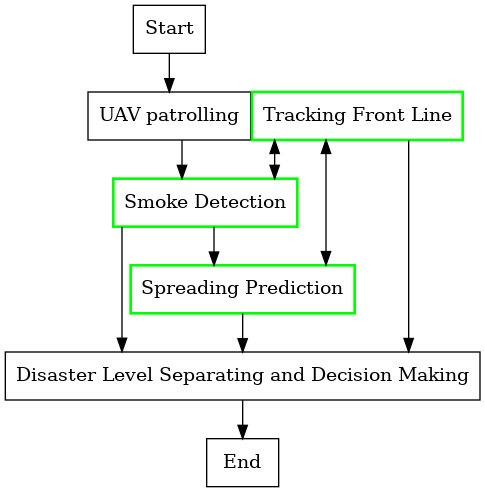
\includegraphics[width=60mm,height=60mm]{figs/arrangement.png}
    \caption{Main process of wildfire fighting using UAV}
    \label{fig:arrangement}
\end{figure}
Encouraged by so many excellent NN-based wildfire fighting strategies in recent years, this research is trying to design and develop a NN-based system with support of UAV and ground work station for early wildfire detection, prediction, and tracking with UAV. Fig.~\ref{fig:arrangement} is the brief structure of the wildfire detection and alarm system which is going to be build in this research. The main contributions could be induced in green boxed items, where they are detection, prediction and tracking. The reminder of the proposal of this research is structured as below:\par 
In Section 2, there are statements of related works and motivation of this research. Section 3 is the description and analysis of objective of this report. Some concepts of the proposed and preparing methodologies are placed in Section 4. Conclusions and potential future works are outlined in Section 5. Timeline and some of research process are illustrated in appendix.\par

\vspace{-0.3cm}
